\documentclass[border=3pt]{standalone}
% Shared preamble for the standalone figures of qurl_explained.tex.
% Build a figure from this folder:   tectonic fig_<name>.tex
% Colours: blue = full precision (FP), orange = 8-bit.
\usepackage[T1]{fontenc}
\usepackage{lmodern}
\usepackage{amsmath,amssymb}
\usepackage[dvipsnames]{xcolor}
\usepackage{tikz}
\usetikzlibrary{positioning,arrows.meta,calc,decorations.pathreplacing}
\usepackage{pgfplots}
\pgfplotsset{compat=1.17}
\colorlet{fp}{RoyalBlue}
\colorlet{qb}{BurntOrange}
\colorlet{good}{ForestGreen}
\colorlet{bad}{BrickRed}
\newcommand{\pold}{\pi_{\mathrm{old}}}
\newcommand{\thold}{\theta_{\mathrm{old}}}
\newcommand{\qthold}{\hat\theta_{\mathrm{old}}}
\tikzset{
  box/.style={draw, rounded corners=3pt, align=center, inner sep=4pt, font=\small},
  arr/.style={-{Stealth[length=2.2mm]}, thick},
  lab/.style={font=\footnotesize, align=center},
}
\pgfplotsset{
  small axes/.style={
    tick label style={font=\footnotesize}, label style={font=\footnotesize},
    title style={font=\small}, every axis plot/.append style={line join=round}},
}

\begin{document}
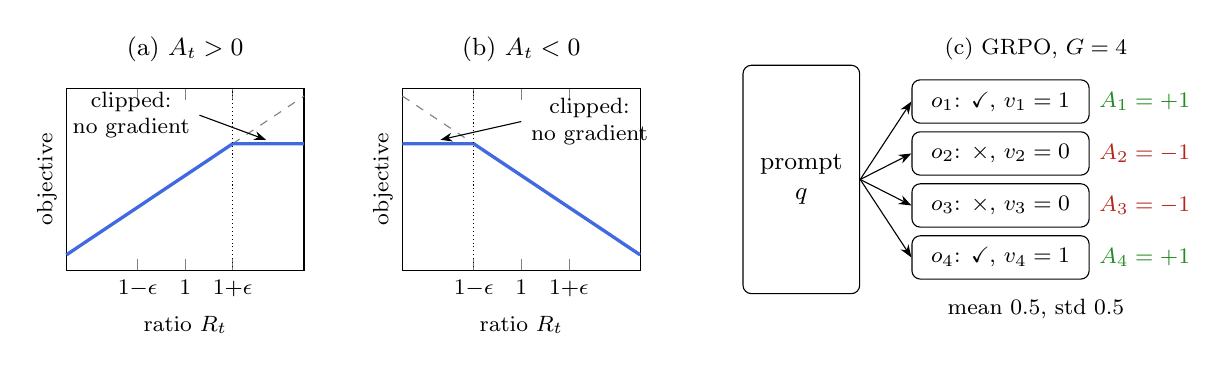
\begin{tikzpicture}
\pgfplotsset{clipax/.style={small axes, width=4.6cm, height=3.9cm, xmin=0.5, xmax=1.5, clip=false,
  xtick={0.8,1,1.2}, xticklabels={$1{-}\epsilon$,$1$,$1{+}\epsilon$}, ytick=\empty,
  xlabel={ratio $R_t$}, ylabel={objective}}}
% (a) positive advantage: objective R_t A_t, capped once R_t > 1 + eps
\begin{axis}[name=pos, clipax, title={(a) $A_t>0$}, ymin=0.4, ymax=1.55]
\addplot[gray, dashed, domain=1.2:1.5] {x};
\addplot[fp, very thick, domain=0.5:1.5, samples=101] {min(x,1.2)};
\draw[densely dotted] (axis cs:1.2,0.4) -- (axis cs:1.2,1.55);
\node[lab, anchor=east] (la) at (axis cs:1.06,1.38) {clipped:\\ no gradient};
\draw[-{Stealth[length=1.5mm]}, thin] (la.east) -- (axis cs:1.34,1.225);
\end{axis}
% (b) negative advantage: objective R_t A_t, floored once R_t < 1 - eps
\begin{axis}[name=neg, clipax, at={($(pos.east)+(1.25cm,0)$)}, anchor=west, title={(b) $A_t<0$}, ymin=-1.6, ymax=-0.45]
\addplot[gray, dashed, domain=0.5:0.8] {-x};
\addplot[fp, very thick, domain=0.5:1.5, samples=101] {-max(x,0.8)};
\draw[densely dotted] (axis cs:0.8,-1.6) -- (axis cs:0.8,-0.45);
\node[lab, anchor=west] (lb) at (axis cs:1.0,-0.66) {clipped:\\ no gradient};
\draw[-{Stealth[length=1.5mm]}, thin] (lb.west) -- (axis cs:0.66,-0.775);
\end{axis}
% (c) GRPO group advantages
\node[box, text width=1.2cm, minimum height=2.9cm, right=1.3cm of neg.east] (q) {prompt\\ $q$};
\foreach \i/\ok/\v/\a/\col [count=\k] in {1/\checkmark/1/+1/good, 2/\times/0/-1/bad, 3/\times/0/-1/bad, 4/\checkmark/1/+1/good} {
  \node[box, anchor=west, minimum width=2.25cm, minimum height=0.55cm, inner sep=2pt, font=\footnotesize]
    (o\i) at ($(q.east)+(0.65cm,1.65cm-\k*0.66cm)$) {$o_{\i}$: $\ok$,\ $v_{\i}=\v$};
  \node[anchor=west, font=\footnotesize, text=\col] at (o\i.east) {$A_{\i}=\a$};
  \draw[-{Stealth[length=1.6mm]}] (q.east) -- (o\i.west);
}
\node[lab, above=0.12cm of o1, xshift=0.45cm] {(c) GRPO, $G=4$};
\node[lab, below=0.12cm of o4, xshift=0.45cm] {mean $0.5$, std $0.5$};
\end{tikzpicture}
\end{document}
